\subsubsection{Rendu avec OpenGL}
L'ensemble des rendus est réalisé avec OpenGL et des shaders écrits en GLSL. Lorsque un objet est chargé dans la scène, le chargeur d'objet remplit des tableaux tels que la position des sommets, les couleurs et les normales associées aux sommets, et les indices associés aux sommets de chaque faces.\\
Le problème est que certains fichiers d'objet, notamment les fichiers avec le format .ply, ne possèdent pas d'information sur les couleurs et les normales des sommets. Or c'est information sont indispensable pour avoir un beau rendu 2D. Ainsi si ces informations sont manquantes, la couleur de l'objet est mise à grise par défaut et les normales sont recalculées à partir de l'orientation des faces.

\subsubsection{Le VAO}
Toutes les informations sur l'objet sont placées dans un VAO (Vertex Array Object) et transmises une seul fois à la carte graphique lors de l'initialisation. Ensuite ce VAO est traité pour chaque rendu par des shaders.\\
Cette technique présente l'avantage d'envoyer le VAO une seul fois à la carte graphique alors qu'avec la méthode du rendu sans shader, les données de l'objet sont envoyées à chaque rendu, ce qui le ralenti considérablement.

\subsubsection{Les shaders}
Sans shaders les rendus n'était pas esthétiques (figure \ref{fig:screenRenduSansShader.png}), l'ombrage n'était pas doux et à la frontière entre chaque face était clairement visible.\\
Les shaders ont pu remédier à cela grace à la technique du \textit{per-pixel lighting} : l'ombrage n'est plus calculé face par face mais pixel par pixel, ce qui offre une plus grande précision et ce qui permet de lisser l'ombre.\\

\begin{figure}[h!]
	\centering
	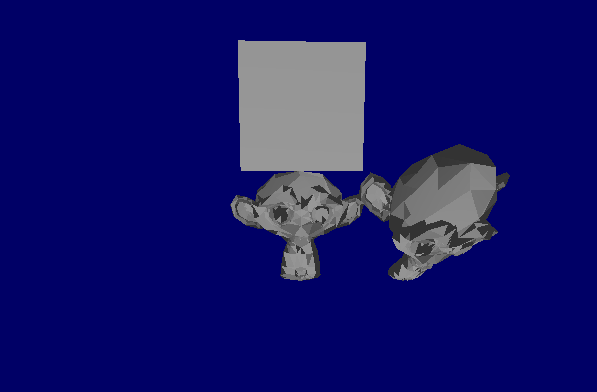
\includegraphics[scale=0.5]{images/rendu_sans_shader.png}
	\caption{\label{fig:screenRenduSansShader.png} Rendu sans shaders qui avait été effectué au debut du developpement du logiciel. L'ombrage est très chaotique. \protect}
\end{figure}

\subsubsection{La spécularité}
Pour améliorer le rendu, il a été choisi de rajouter une spécularité à l'aide du shader. Cette effet permet de simuler les réflections de lumière sur l'objet (figure \ref{fig:screenSpecular.png}). Le shader calcul pour cela la reflection de la lumière sur la surface.


\begin{figure}[h!]
	\centering
	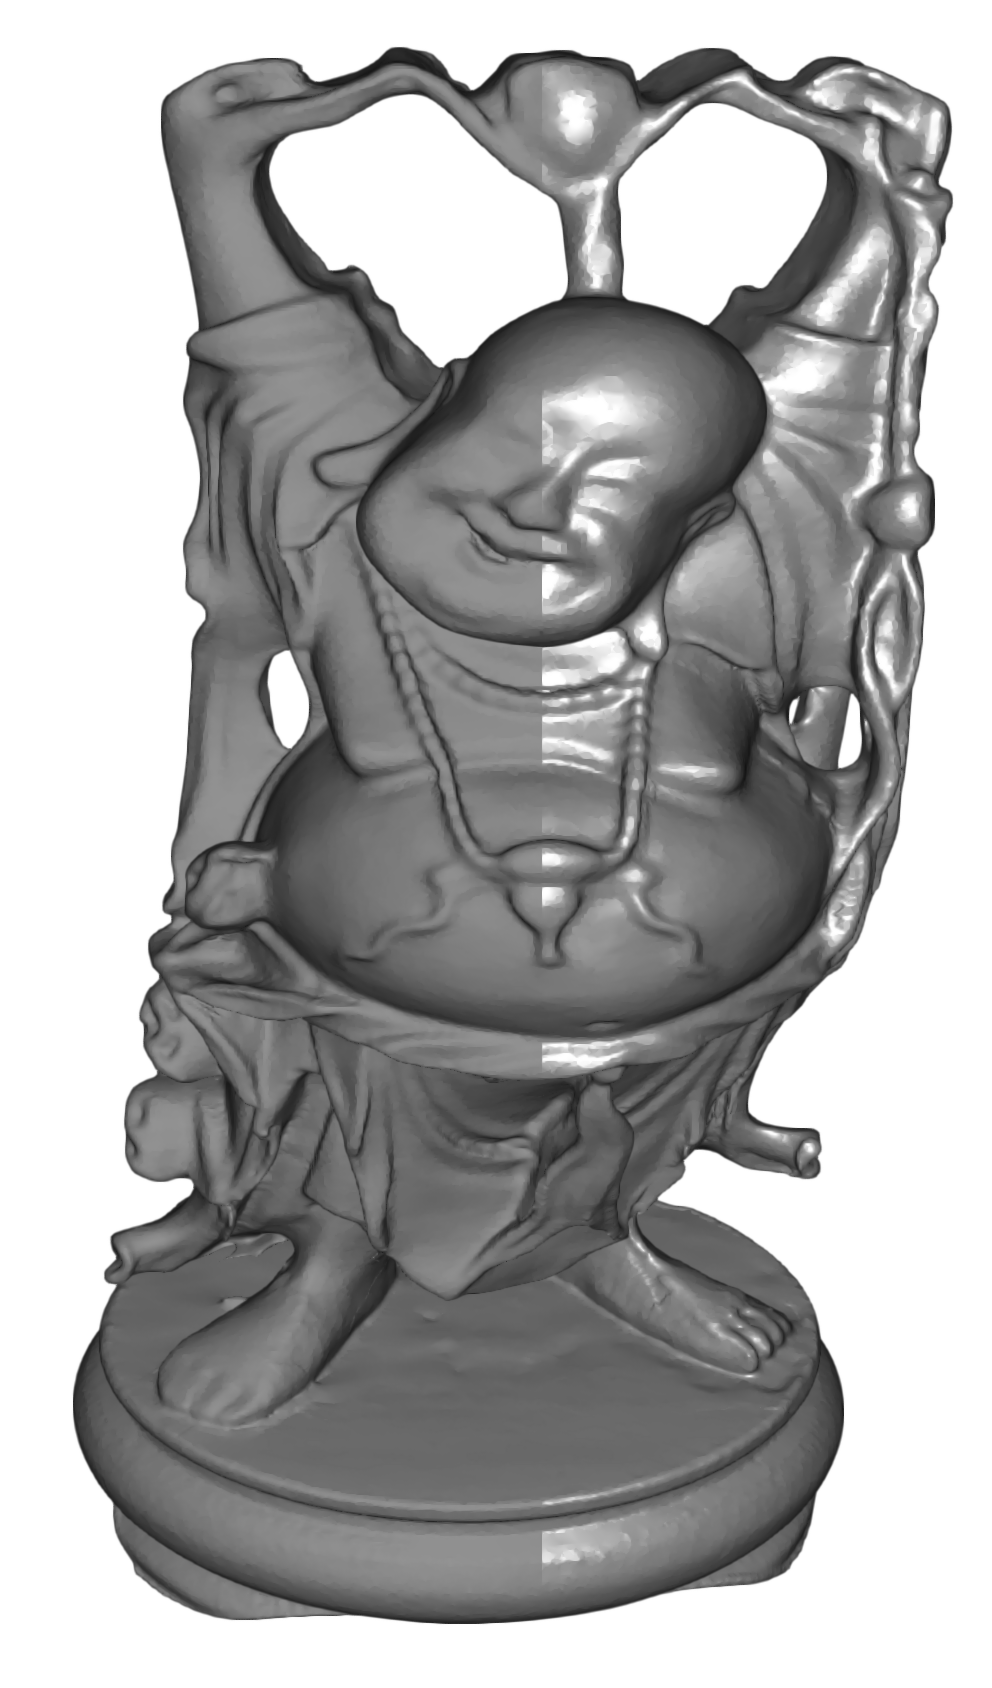
\includegraphics[scale=0.23]{images/rendu_specular.png}
	\caption{\label{fig:screenSpecular.png} Rendu avec l'ombrage de base à gauche et avec la spécularité à droite. \protect}
\end{figure}

\subsubsection{L'anti-aliasing}

\begin{figure}[h!]
	\centering
	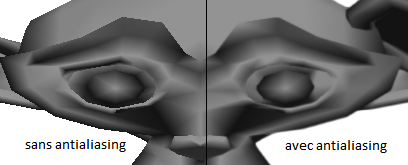
\includegraphics[scale=0.4]{images/antialiasing.png}
	\caption{\label{fig:antialiasing.png} Rendu de base à gauche et avec anti-aliasing à droite. \protect}
\end{figure}

